\chapter{Preconditioning and Subset Selection for Synergistic Reconstruction}
\label{chapter:optimisation}

Chapter~\ref{chapter:wdtnv} defined the smoothed weighted directional total nuclear variation prior. Applying this coupled, edge-preserving prior at scale raises three linked optimisation questions. First, overlapping PET bed positions must be reconstructed into a common image if the prior is to act consistently across their overlap. Second, PET and SPECT subsets can be paired or treated as separate stochastic functions. Third, the very different data and prior curvature scales require an effective preconditioner. This chapter addresses these questions in turn and uses the resulting evidence to motivate the optimisation protocol carried forward into Chapter~\ref{chapter:paper}. That application protocol had already been frozen before the wider preconditioner comparison reported here.

\section{Multi-Bed PET Acquisition}
\label{sec:multibed}

Whole-liver PET commonly requires multiple partially overlapping bed positions. Reconstructing each bed independently and fusing the resulting images is awkward for an edge-preserving prior because the regularisation decisions on either side of the overlap are then made independently. A joint formulation instead estimates one activity image over the combined field of view.

\subsection{Notation}
\label{subsec:multibed_notation}

Let $x$ be the PET activity image on the combined reconstruction grid. For bed position $b=1,\ldots,B$, let $R_b$ restrict the combined image to the axial support reconstructed by bed $b$. The expected PET data for bed $b$ are
\begin{equation}
    \bar y_b(x)
    =
    A_b R_b x + r_b,
    \label{eq:multibed_forward_model}
\end{equation}
where $A_b$ is the bed-specific PET system matrix and $r_b$ collects additive corrections. The joint PET data term is
\begin{equation}
    \mathcal{D}_{\mathrm{PET}}^{\mathrm{multi}}(x)
    =
    \sum_{b=1}^{B}
    \mathcal{D}_b
    \left(
        y_b \mid A_b R_b x + r_b
    \right),
    \label{eq:multibed_data_term}
\end{equation}
with gradient
\begin{equation}
    \nabla \mathcal{D}_{\mathrm{PET}}^{\mathrm{multi}}(x)
    =
    \sum_{b=1}^{B}
    R_b^\top
    A_b^\top
    \nabla_{\bar y_b}
    \mathcal{D}_b
    \left(
        y_b \mid A_b R_b x + r_b
    \right).
    \label{eq:multibed_gradient}
\end{equation}
The corresponding PET sensitivity image on the combined grid is
\begin{equation}
    s_{\mathrm{PET}}^{\mathrm{multi}}
    =
    \sum_{b=1}^{B}
    R_b^\top A_b^\top \bm 1.
    \label{eq:multibed_sensitivity}
\end{equation}
This sensitivity is used in the EM/BSREM data-curvature term in exactly the same way as the single-bed sensitivity in Equation~\eqref{eq:data_hessian_surrogate}.

\subsection{Why Not Stitch Independent Reconstructions?}
\label{subsec:stitching_failure}

A common practical alternative is to reconstruct each PET bed independently and fuse the images using sensitivity-weighted stitching in the overlap. With an edge-preserving prior, however, each reconstruction makes its own noise-suppression and edge decisions before fusion. The qualitative example in Figure~\ref{fig:optim_multibed_qualitative} shows overlap-region noise and discontinuities after separate reconstruction and fusion. It is included to motivate the joint formulation; no quantitative comparison was performed. \TODO{Add the Zenodo-managed citation for the multi-bed PET work.}

\begin{figure}[htbp]
    \centering
    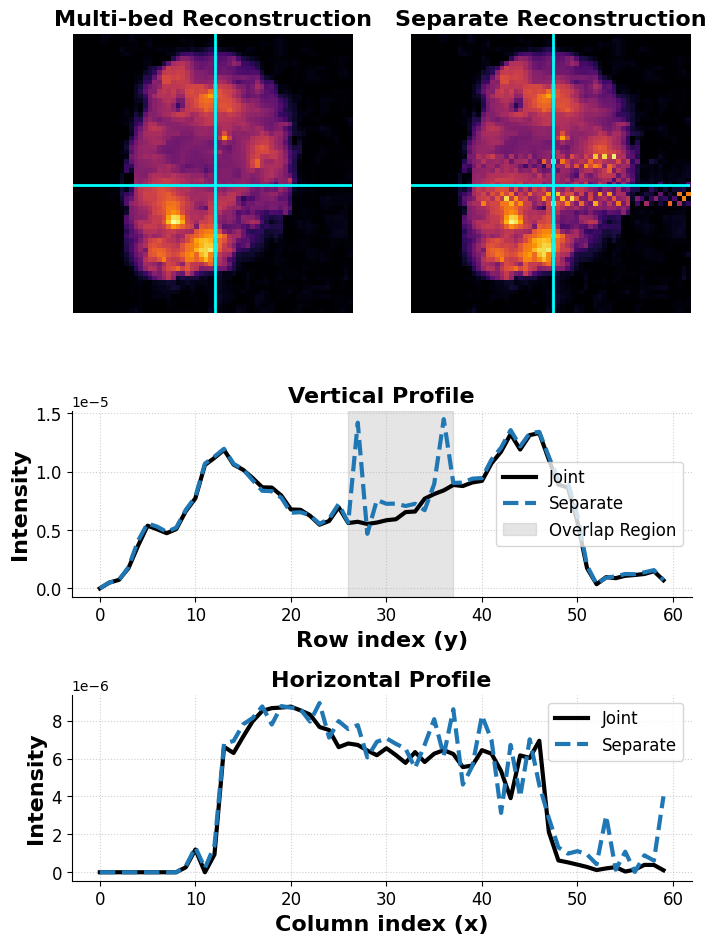
\includegraphics[width=0.72\linewidth]{figures/PiW/comparison.png}
    \caption{Qualitative comparison of separately reconstructed and fused PET bed positions with a joint multi-bed reconstruction using CT-guided edge-preserving regularisation. The shaded region marks the bed overlap and the cyan lines mark the displayed profiles. This example illustrates overlap-region behaviour only; no quantitative comparison was performed.}
    \label{fig:optim_multibed_qualitative}
\end{figure}

\subsection{Joint Reconstruction}
\label{subsec:joint_multibed}

The joint formulation in Equation~\eqref{eq:multibed_data_term} estimates a single combined PET image. Each bed contributes its own data term and sensitivity, while the image-domain prior is evaluated over the complete combined field of view. The combined reconstruction therefore permits the edge-preserving prior to act consistently across the overlap, which is the behaviour required for the dual-bed application in Chapter~\ref{chapter:paper}. This construction does not itself guarantee an artefact-free reconstruction; the evidence here is qualitative.

\section{Stochastic MAP Optimisation}
\label{sec:optimisation_svrg}

Let $\bm z=(z_1,z_2)$ denote the PET and SPECT images represented on a common reconstruction grid. For $N_s$ sampled data functions, define $\mathcal D(\bm z)=\sum_{i=1}^{N_s}\mathcal D_i(\bm z)$. The objective is
\begin{equation}
    \mathcal{O}(\bm z)
    =
    \mathcal D(\bm z)
    +
    \mathcal{R}_{\mathrm{w\text{-}dTNV}}(\bm z)
    +
    \iota_{\mathbb{R}_+}(\bm z),
    \label{eq:optimisation_objective}
\end{equation}
where $\mathcal{D}_i$ is a Poisson negative log-likelihood term composed with the relevant projector, image-space registration operator, and optional resolution model; $\mathcal{R}_{\mathrm{w\text{-}dTNV}}$ is the prior from Chapter~\ref{chapter:wdtnv}; and $\iota_{\mathbb{R}_+}$ enforces non-negativity.

The stochastic experiments use SVRG \cite{johnson_accelerating_2013,twyman_investigation_2022,ehrhardt_fast_2025}. Writing $\mathcal R=\mathcal{R}_{\mathrm{w\text{-}dTNV}}$, the implemented estimator keeps the complete prior outside the sampler. At anchor point $\widetilde{\bm z}$ it is
\begin{equation}
    g^{(k)} = \nabla\mathcal R(\bm z^{(k)})
    + \nabla\mathcal D(\widetilde{\bm z})
    + N_s\!\left[
        \nabla\mathcal D_{i_k}(\bm z^{(k)})
        -\nabla\mathcal D_{i_k}(\widetilde{\bm z})
    \right],
    \qquad i_k\sim\operatorname{Unif}\{1,\ldots,N_s\}.
    \label{eq:svrg_estimator_general}
\end{equation}
The data functions are sampled uniformly with replacement. The complete prior gradient is evaluated at every stochastic update, and the full data-gradient snapshot is refreshed once per epoch.

The image update is a projected, preconditioned gradient step,
\begin{equation}
    \bm z^{(k+1)}
    =
    \left\{
    \bm z^{(k)}
    -
    \varsigma^{(k)} P^{(k)} g^{(k)}
    \right\}_{\geq 0},
    \label{eq:optimisation_projected_update}
\end{equation}
where $P^{(k)}$ is either a diagonal preconditioner or a voxel-wise $2\times2$ block preconditioner coupling the PET and SPECT update components. The step size follows the linear decay rule
\begin{equation}
    \varsigma^{(k)}
    =
    \frac{\varsigma^{(0)}}{1+\eta_{\mathrm{relax}} k},
    \qquad
    \varsigma^{(0)}=1,
    \qquad
    \eta_{\mathrm{relax}}=0.002,
    \label{eq:optimisation_step_size}
\end{equation}
for the 20-pass comparisons described below.

\subsection{Common Evaluation Protocol}
\label{subsec:optimisation_evaluation_protocol}

The convergence experiments used an anthropomorphic phantom scanned on the Mediso AnyScan at the National Physical Laboratory. PET and SPECT were each partitioned into 18 subsets. Each plotted comparison curve comprises five stochastic realisations and covers the first 20 complete data passes. A single 1000-epoch reconstruction of the same objective, run with more conservative optimisation settings, provided the reference image $x^\star$; it is a final long-run iterate rather than a known global minimiser.

For each stochastic run and each saved iteration, the \acrfull{nrmse} in region $R$ is
\begin{equation}
    \operatorname{NRMSE}(x_k,x^\star;R)
    =
    \frac{\sqrt{N^{-1}\sum_{j\in R}(x_{k,j}-x^\star_j)^2}}
         {\sqrt{N^{-1}\sum_{j\in R}(x^\star_j)^2}},
    \qquad N=|R|.
    \label{eq:optimisation_nrmse}
\end{equation}
The regions are evaluated separately over the whole image, the hot-sphere mask, and the cold-sphere mask. The plotted centre line is the arithmetic mean of the five per-run NRMSE values at each iteration, not the NRMSE of an averaged reconstruction; the envelope is their pointwise minimum--maximum. The long-run reference itself was generated once.

\section{Prior-Aware Preconditioning}
\label{sec:optimisation_preconditioners}
\label{subsec:preconditioning}

Preconditioning is critical for subset-based MAP reconstruction because the data term and the edge-preserving prior can have very different local curvature scales \cite{clinthorne_preconditioning_1993,ahn_globally_2002,de_pierro_fast_2001,ehrhardt_fast_2025}. The current experiments compare data-only BSREM scaling with several prior-aware curvature surrogates for $\wdtnv$.

\subsection{Data Curvature}
\label{subsec:optimisation_data_preconditioning}

For modality $m$, let $s_m$ denote the sensitivity image on the shared grid,
\begin{equation}
    s_m
    =
    W_m A_m^\top \bm 1,
    \label{eq:shared_grid_sensitivity}
\end{equation}
where $A_m$ is the native-grid system matrix and $W_m$ maps native images to the shared prior grid. The EM/BSREM data preconditioner is
\begin{equation}
    P_{\mathrm{BSREM},m}
    =
    (z_m+\epsilon_x)\oslash s_m,
    \label{eq:bsrem_preconditioner}
\end{equation}
with element-wise division. Equivalently, the corresponding diagonal data Hessian surrogate is
\begin{equation}
    \widehat H_{\mathrm{data},m}
    =
    s_m \oslash (z_m+\epsilon_x).
    \label{eq:data_hessian_surrogate}
\end{equation}
The implementation optionally smooths the numerator image used in the EM preconditioner with a Gaussian filter. In the experiments below the smoothing FWHM is $5\,\mathrm{mm}$ in each direction.

\subsection{Current \texorpdfstring{$\wdtnv$}{w-dTNV} Prior Curvature}
\label{subsec:optimisation_prior_preconditioning}

The current prior-aware preconditioners use the \acrfull{mm}/\acrfull{irls} curvature implied by the smoothed spectral penalty. At voxel $n$, let
\begin{equation}
    Y_n
    =
    \left[
        \beta_{1,n}\Pi_{1,n}(Dz_1)_n
        \;\middle|\;
        \beta_{2,n}\Pi_{2,n}(Dz_2)_n
    \right]\in\mathbb{R}^{d\times2}
    \label{eq:optimisation_weighted_jacobian}
\end{equation}
be the weighted directional Jacobian from Chapter~\ref{chapter:wdtnv}. The active code forms the modality-space \glsentryshort{mm} weight
\begin{equation}
    C_n
    =
    \left(Y_n^\top Y_n + \epsilon^2 I_2\right)^{-1/2}
    =
    \begin{pmatrix}
        c_{11,n} & c_{12,n}\\
        c_{12,n} & c_{22,n}
    \end{pmatrix}.
    \label{eq:mm_weight_current_code}
\end{equation}
This matrix is the same $2\times2$ inverse square-root used in the gradient calculation, now interpreted as the local quadratic-surrogate weight.

For diagonal preconditioning, the finite-difference stencil and directional projectors are collapsed to a per-voxel participation factor $\tau_{m,n}$. This factor includes the number of valid forward/backward stencil incidences at voxel $n$, the squared finite-difference scale factors, and the diagonal entries of $\Pi_{m,n}^\top\Pi_{m,n}$. The local diagonal \wdtnv{} curvature approximation is
\begin{equation}
    \widehat H_{\mathcal R,m,n}^{\mathrm{loc\text{-}diag}}
    =
    V_{\mathrm{vox}}\,
    \beta_{m,n}^2\,c_{mm,n}\,\tau_{m,n}.
    \label{eq:diag_tight_preconditioner}
\end{equation}
This is the diagonal extraction of the local \glsentryshort{mm} curvature surrogate, and is therefore an approximation rather than a strict Loewner majoriser in general. The Gershgorin diagonal majoriser inflates the modality-space diagonal by the absolute off-diagonal coupling,
\begin{equation}
    \widehat H_{\mathcal R,1,n}^{\mathrm{diag\text{-}G}}
    =
    V_{\mathrm{vox}}\,
    \beta_{1,n}^2\,(c_{11,n}+|c_{12,n}|)\,\tau_{1,n},
    \qquad
    \widehat H_{\mathcal R,2,n}^{\mathrm{diag\text{-}G}}
    =
    V_{\mathrm{vox}}\,
    \beta_{2,n}^2\,(c_{22,n}+|c_{12,n}|)\,\tau_{2,n}.
    \label{eq:diag_gersh_preconditioner}
\end{equation}

For block preconditioning, the PET and SPECT update components at each voxel are coupled by a $2\times2$ block. Let $\mathcal{N}(n)$ be the set of target voxels whose finite-difference stencil depends on source voxel $n$. For target voxel $r\in\mathcal{N}(n)$, let $c_{r\leftarrow n}\in\mathbb{R}^d$ be the finite-difference impulse vector produced in the directional channels when source voxel $n$ is perturbed. The local voxel-block curvature approximation uses
\begin{equation}
    \alpha_{r\leftarrow n}^{mm'}
    =
    c_{r\leftarrow n}^\top
    \Pi_{m,r}^\top
    \Pi_{m',r}
    c_{r\leftarrow n},
    \label{eq:block_alpha}
\end{equation}
and
\begin{equation}
    \widehat H_{\mathcal R,n}^{\mathrm{loc\text{-}block}}
    =
    V_{\mathrm{vox}}
    \sum_{r\in\mathcal{N}(n)}
    \left[
        B_r C_r B_r
    \right]
    \circ
    A_{r\leftarrow n},
    \qquad
    A_{r\leftarrow n}
    =
    \begin{pmatrix}
        \alpha_{r\leftarrow n}^{11} & \alpha_{r\leftarrow n}^{12}\\
        \alpha_{r\leftarrow n}^{21} & \alpha_{r\leftarrow n}^{22}
    \end{pmatrix},
    \label{eq:block_tight_preconditioner}
\end{equation}
where $B_r=\mathrm{diag}(\beta_{1,r},\beta_{2,r})$ and $\circ$ denotes the Hadamard product. The long reference reconstructions in the subset-selection study use a more conservative voxel-block curvature majoriser.

\subsection{Combining Data and Prior Curvature}
\label{subsec:optimisation_preconditioner_combination}

The current experiments invert the summed data and prior Hessian surrogates. For diagonal methods,
\begin{equation}
    P_{m,n}^{\mathrm{diag}}
    =
    \left(
        \widehat H_{\mathrm{data},m,n}
        +
        \widehat H_{\mathcal R,m,n}
    \right)^{-1},
    \label{eq:diag_majoriser_combination}
\end{equation}
with numerical floors and optional maximum-value caps. For block methods,
\begin{equation}
    P_{n}^{\mathrm{block}}
    =
    \left(
        \begin{pmatrix}
        \widehat H_{\mathrm{data},1,n} & 0\\
        0 & \widehat H_{\mathrm{data},2,n}
        \end{pmatrix}
        +
        \widehat H_{\mathcal R,n}
    \right)^{-1}.
    \label{eq:block_majoriser_combination}
\end{equation}
This differs from the application implementation in Chapter~\ref{chapter:paper}, where the same local diagonal \wdtnv{} curvature approximation was combined with the data preconditioner using a Lehmer mean.

The preconditioner is updated once per epoch in the experiments unless an explicit update interval is supplied. Between updates the curvature is therefore stale, which is a pragmatic compromise between optimisation stability and the computational cost of evaluating $\widehat H_{\mathcal R}$.

\begin{table}[htbp]
\centering
\caption{Preconditioner settings used in the current preconditioner experiments.}
\label{tab:preconditioner_settings}
\begin{tabular}{lll}
\toprule
Preconditioner setting & Prior curvature model & Combination used in sweep\\
\midrule
Data-only EM/BSREM scaling & none & none\\
Local diagonal \wdtnv{} curvature approximation & diagonal extraction of local \glsentryshort{mm} curvature & Hessian-sum inversion\\
Gershgorin diagonal \wdtnv{} curvature majoriser & diagonal majoriser including cross-modal coupling & Hessian-sum inversion\\
Local voxel-block \wdtnv{} curvature approximation & voxel-wise $2\times2$ local \glsentryshort{mm} curvature & Hessian-sum inversion\\
Conservative voxel-block \wdtnv{} curvature majoriser & voxel-wise $2\times2$ conservative majoriser & reference runs\\
\bottomrule
\end{tabular}
\end{table}

\subsection{Preconditioner Comparison Methods}
\label{subsec:preconditioner_experiment_methods}

Four preconditioner settings are compared: data-only BSREM, the local diagonal \wdtnv{} curvature approximation, the Gershgorin diagonal \wdtnv{} curvature majoriser, and the local voxel-block \wdtnv{} curvature approximation. These settings are summarised in Table~\ref{tab:preconditioner_settings}.

All sweep reconstructions use the same objective, prior settings, and initialisation within each dataset. The fixed sweep parameters are $\alpha=\beta=1$, $\gamma_{\mathrm{TNV}}=0.02$, initial step size $\varsigma^{(0)}=1$, relaxation parameter $\eta_{\mathrm{relax}}=0.002$, and $25$ epochs. Time-of-flight PET is disabled in these optimisation experiments. Sensitivity-derived support masks are enabled with relative threshold $10^{-3}$, and both EM and prior-aware preconditioner maximum-value caps are disabled. The EM component of the preconditioner is smoothed with a $5\,\mathrm{mm}$ Gaussian FWHM.

Experiments are configured for a single-bed anthropomorphic phantom dataset and a two-bed clinical PET/SPECT dataset. For the one-bed sweep, the reconstruction is routed through the subset-selection runner with separate PET/SPECT subset functions and the prior evaluated deterministically every iteration. The two-bed sweep uses the corresponding two-bed reconstruction path. Objective values, saved images, and convergence metrics are recorded for comparison against long-run reference reconstructions. The corresponding numerical comparisons are reported below.

\section{Subset Selection}
\label{sec:optimisation_subset_selection}

Subset methods accelerate early iterations in emission tomography by replacing full data passes with stochastic or ordered blocks of projection data \cite{hudson_accelerated_1994}. In synergistic PET/SPECT reconstruction there is an additional design choice: PET, SPECT, and the coupled prior can be grouped together or sampled separately. Previous work on synergistic subset selection \cite{porter_optimising_2024}\TODO{Zenodo-managed bibliography entry pending for \texttt{porter\_optimising\_2024}; IEEE Xplore document 10654962.} motivated a more systematic comparison of these choices under the current SVRG and preconditioning implementation.

\subsection{Data-Subset Organisation}
\label{subsec:subset_data_organisation}

Two data-subset organisations are tested.

\paragraph{Separate subsets.}
PET and SPECT subsets are treated as distinct stochastic functions. For a one-bed acquisition with $N_{\mathrm{PET}}=18$ and $N_{\mathrm{SPECT}}=18$, this gives
\begin{equation}
    \{\mathcal{D}_i\}_{i=1}^{36}
    =
    \{
    \mathcal{D}_{\mathrm{PET},1},\ldots,\mathcal{D}_{\mathrm{PET},18},
    \mathcal{D}_{\mathrm{SPECT},1},\ldots,\mathcal{D}_{\mathrm{SPECT},18}
    \}.
    \label{eq:separate_subset_functions}
\end{equation}
For a two-bed PET acquisition with $9$ PET subsets per bed and $9$ SPECT subsets, the separate list contains $27$ data functions: $18$ PET bed-specific functions and $9$ SPECT functions.

\paragraph{Paired subsets.}
PET and SPECT subsets with matching indices are summed into one stochastic function. For one bed this gives
\begin{equation}
    \mathcal{D}^{\mathrm{pair}}_j
    =
    \mathcal{D}_{\mathrm{PET},j}
    +
    \mathcal{D}_{\mathrm{SPECT},j},
    \qquad j=1,\ldots,18.
    \label{eq:paired_subset_functions}
\end{equation}
For two PET beds, each paired function contains both PET bed-position subsets and the corresponding SPECT subset,
\begin{equation}
    \mathcal{D}^{\mathrm{pair}}_j
    =
    \mathcal{D}_{\mathrm{PET},1,j}
    +
    \mathcal{D}_{\mathrm{PET},2,j}
    +
    \mathcal{D}_{\mathrm{SPECT},j},
    \qquad j=1,\ldots,9.
    \label{eq:paired_subset_functions_2bpos}
\end{equation}
The two-bed paired mode therefore requires equal PET and SPECT subset counts after partitioning.

\subsection{Prior Sampling Strategy}
\label{subsec:subset_prior_strategy}

The prior is handled in two ways. In \emph{always} mode, the prior gradient is evaluated deterministically on every stochastic iteration and is not part of the sampler. In \emph{subset} mode, the prior is appended as an additional stochastic function and is sampled with a prescribed probability.

Let $N_{\mathrm d}$ be the number of stochastic data functions after the selected data grouping, and let $u$ be the target number of prior updates per data epoch. The implemented prior-sampling probability is
\begin{equation}
    p_{\mathcal R}
    =
    \frac{u}{N_{\mathrm d}+u},
    \label{eq:prior_sampling_probability}
\end{equation}
and each data function probability is scaled by $1-p_{\mathcal R}$. The epoch length is adjusted to
\begin{equation}
    K
    =
    \left\lceil
    \frac{N_{\mathrm d}}{1-p_{\mathcal R}}
    \right\rceil.
    \label{eq:subset_epoch_length}
\end{equation}
For paired mode the default is $u=N_{\mathrm d}$, so the prior and data aggregate each receive probability $1/2$. For separate mode the default is $u=N_{\mathrm d}/2$, so the prior receives probability $1/3$ and the data aggregate receives probability $2/3$. These defaults keep the number of expected prior updates comparable to the paired setting while avoiding a prior update after every separate PET or SPECT subset.

\subsection{Subset-Selection Experiment Methods}
\label{subsec:subset_selection_experiment_methods}

The main subset-selection sweep crosses two subset organisations (\texttt{separate}, \texttt{paired}), two prior modes (\texttt{always}, \texttt{subset}), two preconditioner settings (data-only BSREM and the local diagonal \wdtnv{} curvature approximation), and the configured directional strength $\gamma_{\mathrm{TNV}}=0.02$. The one-bed configuration uses $18$ PET and $18$ SPECT subsets. The two-bed configuration uses $9$ PET subsets per bed position and $9$ SPECT subsets.

All subset-selection runs use SVRG with random-with-replacement sampling, a snapshot interval equal to one adjusted epoch, $\alpha=\beta=1$, initial step size $1$, relaxation parameter $0.002$, and $25$ epochs. The prior is the directional TNV variant with a six-direction stencil, Neumann boundary conditions, Charbonnier smoothing, and no additional modality-specific priors. Sensitivity-derived support masks are enabled, and the EM preconditioner component is smoothed with a $5\,\mathrm{mm}$ Gaussian FWHM. The random seed is fixed at $42$ for reproducibility.

Long-run reference reconstructions are generated using separate subset organisation, deterministic prior evaluation every iteration, the conservative voxel-block \wdtnv{} curvature majoriser, and $1000$ epochs. The results below compare objective histories and image-domain errors against these references at matched data-pass counts.

\section{Conclusion}
\label{sec:optimisation_conclusion}

This chapter has separated the optimisation machinery from the definition of the $\wdtnv$ prior itself. The current preconditioner experiments compare BSREM scaling with \glsentryshort{mm}-derived prior-aware diagonal and block curvature surrogates, combined through Hessian-sum inversion in the active reconstruction code. The subset-selection experiments independently vary modality grouping and prior sampling, including a two-bed PET setting where the data term is evaluated jointly over bed positions. These methods provide the framework into which numerical convergence and image-quality results can be inserted once available.
